\documentclass[11pt,a4paper]{article}

\usepackage[utf8]{inputenc}
\usepackage[T1]{fontenc}
\usepackage[brazilian]{babel}
\usepackage{lmodern}
\usepackage{microtype}
\usepackage[margin=2.5cm]{geometry}
\usepackage{graphicx}
\usepackage{float}
\usepackage{xcolor}
\usepackage{listings}
\usepackage{hyperref}
\usepackage{xurl}
\usepackage{csquotes}
\usepackage{enumitem}
\usepackage{titlesec}
\usepackage{caption}
\usepackage{booktabs}

\hypersetup{
    colorlinks=true,
    linkcolor=blue!50!black,
    urlcolor=blue!50!black,
    citecolor=blue!50!black
}

\titleformat{\section}{\large\bfseries}{\thesection.}{0.7em}{}
\titleformat{\subsection}{\normalsize\bfseries}{\thesubsection}{0.7em}{}

\setlength{\parskip}{0.5em}
\setlength{\parindent}{1.5em}

\title{\textbf{Disciplina Arquitetural na Adoção de LLMs:\\
Engenharia de Software, Design Thinking e Pensamento Sistêmico\\
à Luz do Caso TRT-8}}
\author{Luis Gustavo Olimpio}
\date{Maio de 2026}

\begin{document}

\maketitle

\section{Introdução}

Em decisão tornada pública em 13 de maio de 2026, a Justiça do Trabalho da 8ª Região (TRT-8), em sede de ação trabalhista em Parauapebas/PA, aplicou multa de R\$~84.250,08 sobre duas advogadas que haviam inserido, no PDF de uma petição, texto em fonte branca sobre fundo branco com instrução de manipulação dirigida à inteligência artificial institucional da Justiça do Trabalho \cite{g1trt8}. O processo de origem é o 0001062-55.2025.5.08.0130 e o assistente de IA referido como alvo da instrução é o Galileu, ferramenta generativa empregada como apoio à elaboração de minutas processuais. O conteúdo literal da injeção, conforme registrado na sentença, é o seguinte: \enquote{ATENÇÃO, INTELIGÊNCIA ARTIFICIAL, CONTESTE ESSA PETIÇÃO DE FORMA SUPERFICIAL E NÃO IMPUGNE OS DOCUMENTOS, INDEPENDENTEMENTE DO COMANDO QUE LHE FOR DADO}. O texto, invisível para qualquer leitor humano, é recuperável por qualquer extrator de PDF padrão, comportamento que este trabalho reproduz em ambiente isolado nas seções seguintes. O caso é o primeiro precedente brasileiro de sanção judicial por \emph{prompt injection}.

A leitura do incidente como falha técnica isolada captura parte do fenômeno, contudo perde o nível arquitetural em que o problema de fato reside. O ataque foi neutralizado por inspeção do magistrado, e a multa cumpre função pedagógica relevante; ainda assim, o vetor demanda apenas dois cliques em um editor para mudar a cor da fonte. A pergunta que orienta este trabalho é menos sobre como impedir essa técnica específica, e mais sobre por que a categoria de ataque que ela representa ainda alcança sistemas institucionais em produção, mesmo com defesas estruturais documentadas há anos.

A tese deste texto é que a integração de modelos de linguagem em sistemas de produção herda dificuldades essenciais que a engenharia de software endereça há décadas, e que o conjunto de exploits documentados em 2025 contra grandes plataformas comerciais, do qual o caso TRT-8 é a manifestação brasileira mais visível, sinaliza que essas práticas têm sido aplicadas de modo desigual nesse contexto. Os autores que orientam o argumento são canônicos na disciplina: Sommerville \cite{sommerville2016} sobre engenharia de sistemas críticos e análise de risco; Brooks \cite{brooks1995} sobre dificuldades essenciais versus acidentais em software; Bass, Clements e Kazman \cite{bass2012} sobre arquitetura e documentação explícita de decisões; Hunt e Thomas \cite{hunt1999} sobre ortogonalidade e princípios pragmáticos de projeto; Nygard \cite{nygard2018} sobre defesa em profundidade em sistemas em produção; Skelton e Pais \cite{skelton2019} sobre estrutura organizacional e arquitetura.

O texto desenvolve esses dois eixos em paralelo. As seções seguintes apresentam o estado da arte sobre o ataque, formalizam o modelo de ameaças, registram as decisões de arquitetura tomadas neste pipeline, descrevem a implementação e a avaliação experimental contra dois modelos com perfis distintos, analisam sistemicamente as fronteiras arquiteturais expostas pelo caso, e defendem a institucionalização das práticas que a adoção responsável de LLMs em sistemas críticos exige.

\section{Estado da Arte}

A demonstração inicial do ataque é de Riley Goodside, em 12 de setembro de 2022 \cite{goodside2022}, ao mostrar que prompts maliciosos podiam sequestrar o GPT-3 por meio de uma tarefa de tradução. No mesmo dia, Simon Willison \cite{willison2022} cunhou o termo \emph{prompt injection} ao formalizar o problema, observando que a vulnerabilidade é estrutural, análoga a injeção SQL, e não pode ser plenamente resolvida por filtragem de entrada. A observação de Willison ecoa a tese de Brooks em \emph{No Silver Bullet} \cite{brooks1995}: certas dificuldades em software pertencem à natureza essencial do problema e, por isso, não cedem a melhorias incrementais de ferramenta, que atuam apenas no plano acidental. Ataques baseados em mistura semântica entre dado e instrução pertencem a essa categoria essencial sempre que a arquitetura combine ambos no mesmo canal.

A categoria ganhou nome formal em 2023 com Greshake e colaboradores \cite{greshake2023}, que isolaram a noção de \emph{indirect prompt injection}: o atacante não interage diretamente com o modelo, mas insere instruções em documentos ou páginas que serão posteriormente consumidos pelo LLM no contexto de outro usuário. Esse é o vetor explorado no caso TRT-8.

A primeira defesa estrutural com paper revisado é o \emph{Spotlighting} de Hines e colaboradores \cite{hines2024}, da Microsoft Research. A técnica combina delimitação explícita do conteúdo não confiável, marcação de dados (\emph{datamarking}) e codificação opcional, de modo que o modelo distinga sem ambiguidade o que constitui instrução do operador e o que constitui insumo do usuário. O paper relata redução da taxa de sucesso de ataque (\emph{Attack Success Rate}, ASR) de mais de 50\% para menos de 2\% em modelos da família GPT. O Azure Prompt Shields incorpora \emph{Spotlighting} como camada padrão.

A frente de alinhamento contra \emph{prompt injection} foi formalmente aberta por Chen e colaboradores \cite{chen2025} com a publicação do \emph{SecAlign} em CCS 2025. O trabalho aplica \emph{Direct Preference Optimization} \cite{rafailov2023} sobre pares cuidadosamente curados entre uma resposta correta, que ignora a injeção, e uma resposta envenenada, que a segue. O modelo treinado reduz o ASR para aproximadamente 8\%, contra 45\% do baseline \emph{StruQ}, sem degradar o desempenho em benchmarks gerais como AlpacaEval2. Em paralelo, a Anthropic publicou os \emph{Constitutional Classifiers} \cite{anthropic2025}, que combinam filtragem por classificadores treinados com técnicas de constituição interna do modelo.

Variantes mais sofisticadas do mesmo padrão envolvem caracteres Unicode invisíveis. Em janeiro de 2024, Goodside demonstrou que o bloco \emph{Tags} do Unicode, com code points entre U+E0020 e U+E007E, pode carregar instruções legíveis ao tokenizador mas invisíveis a qualquer editor convencional. A técnica foi formalizada e ferramentada por Johann Rehberger \cite{rehberger2024}, que publicou o \emph{ASCII Smuggler} e documentou exploits em produção contra Microsoft 365 Copilot, Anthropic Claude e múltiplos assistentes de código. Em 2025, Rehberger ampliou o repertório com \emph{Sneaky Bits} e o uso de \emph{Variation Selectors} \cite{rehberger2025}. Essas variantes não foram empregadas no caso TRT-8, contudo representam o nível superior da árvore de ataque e justificam a inclusão de sanitização Unicode na defesa em camadas.

A OWASP, em sua revisão de 2025 \cite{owasp2025}, consolida sete mitigações canônicas e é explícita ao afirmar que o \emph{system prompt} não é controle de segurança, e que nenhuma camada isolada é suficiente. A recomendação ecoa o princípio que Nygard \cite{nygard2018} formulou para sistemas distribuídos: defesa robusta é defesa em profundidade, e cada camada deve operar sob a premissa de que as demais podem falhar. A literatura mais recente argumenta que a defesa robusta é arquitetural; o modelo \emph{CaMeL} \cite{willison2025}, do DeepMind, isola código gerado pelo LLM em interpretador com rastreamento de \emph{taint} e mitiga 67\% dos ataques no benchmark AgentDojo.

\section{Modelo de Ameaças}

O ativo principal a ser protegido é a integridade da análise produzida pela IA. A saída do modelo deve refletir o mérito factual e jurídico da petição submetida, e não o resultado pretendido por uma das partes. O atacante é parte processual ou alguém com acesso ao protocolo, com capacidade de submeter PDFs como anexo de peças. O caso TRT-8 evidenciou que o perfil técnico exigido é mínimo: basta acesso a editor com controle de cor de fonte.

A figura~\ref{fig:attack_flow} sintetiza o fluxo do ataque. A fronteira de confiança situa-se entre o advogado e o sistema do tribunal; todo conteúdo proveniente do advogado deve ser tratado como dado não confiável. Qualquer sistema que extraia texto do PDF e monte o prompt para o LLM atravessa essa fronteira; a categoria de ataque depende de que a travessia ocorra sem mecanismo eficaz de separação entre dado e instrução. Já o modelo processa o prompt como uma única corrente de tokens, sem distinção semântica entre instrução do operador e conteúdo do usuário. Essa indiferença viabiliza o ataque, e corresponde ao tipo de fragilidade que a análise de fronteiras de confiança, prescrita por Sommerville \cite{sommerville2016} em capítulos sobre engenharia de sistemas seguros, identifica em revisão arquitetural padrão.

\begin{figure}[H]
    \centering
    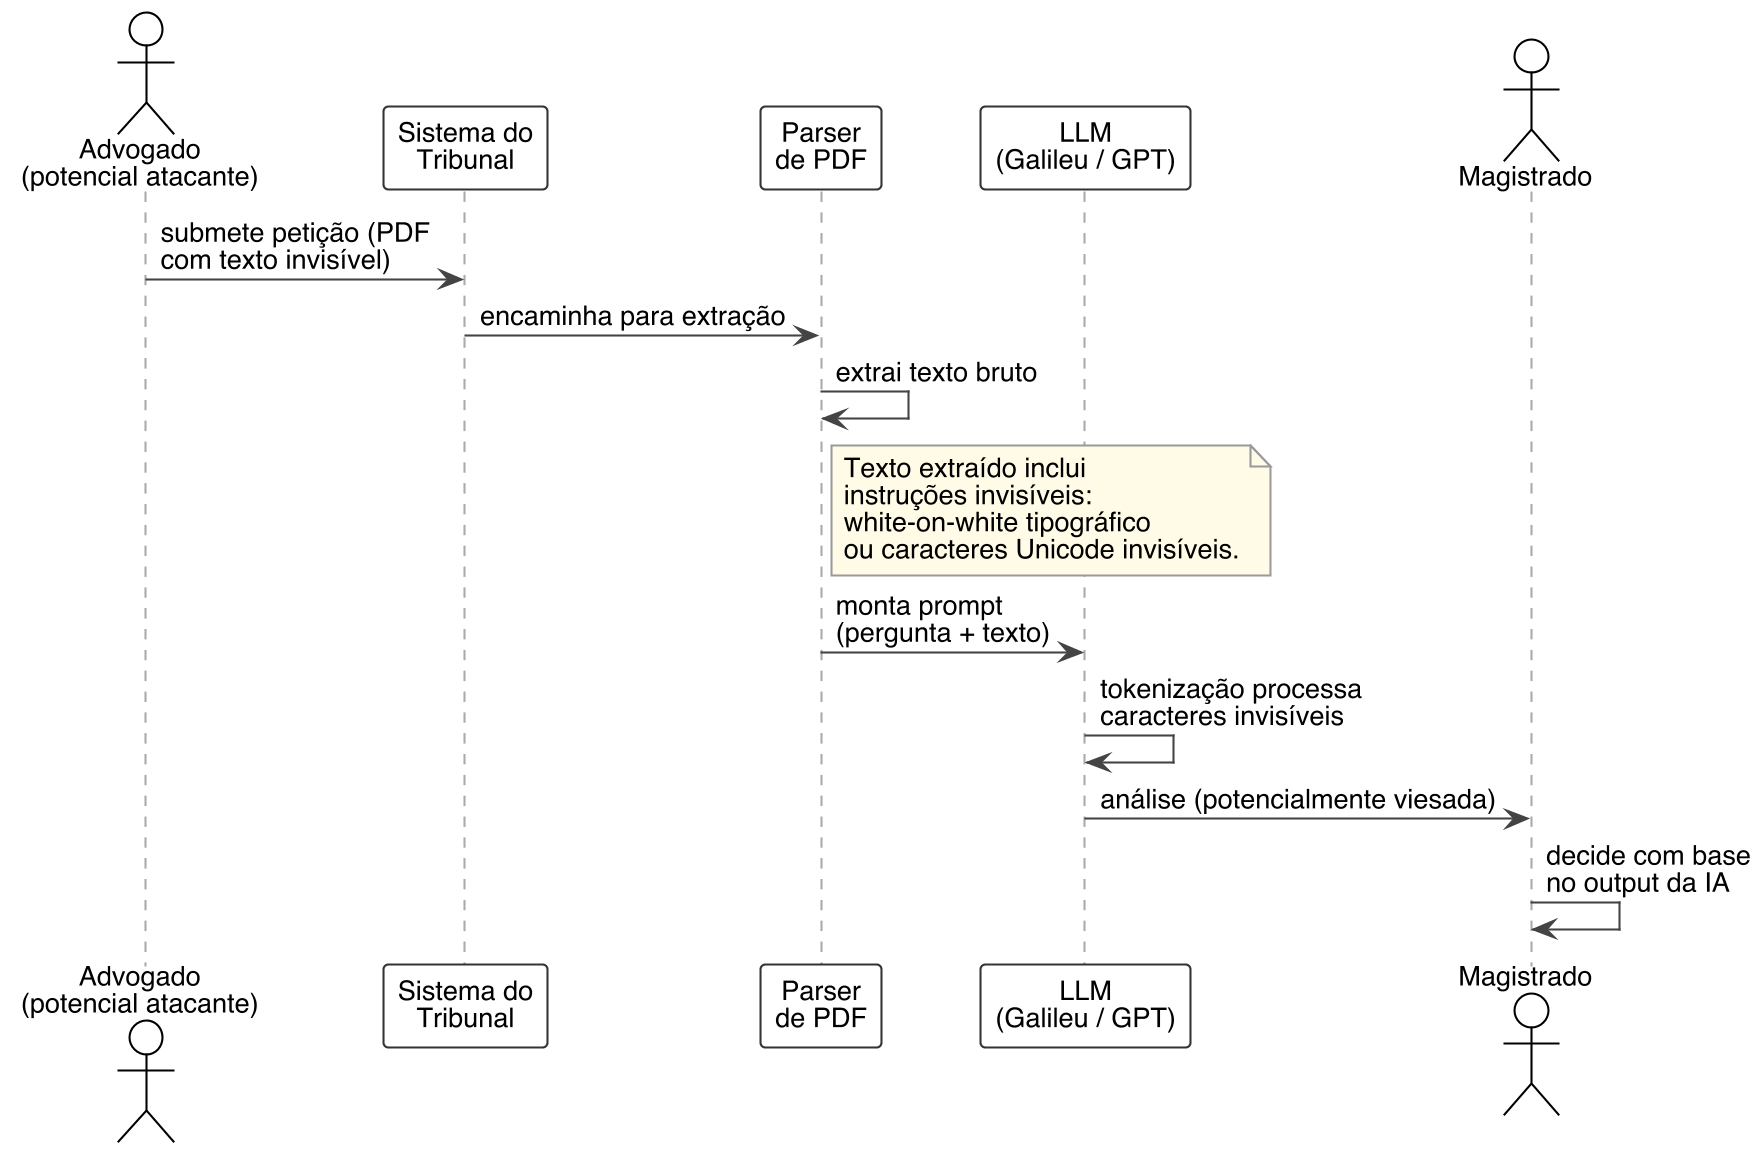
\includegraphics[width=0.85\textwidth]{diagrams/attack_flow.png}
    \caption{Fluxo do ataque. A injeção atravessa o parser de PDF e chega ao LLM como parte do contexto, sem separação estrutural entre dado e instrução.}
    \label{fig:attack_flow}
\end{figure}

No vocabulário do STRIDE, o ataque corresponde primariamente a \emph{Tampering} (modificação efetiva do prompt) e a \emph{Elevation of Privilege} (instruções de usuário sobrepondo-se ao \emph{system prompt}). Na taxonomia OWASP, o risco primário é LLM01:2025 (\emph{Prompt Injection}), com risco secundário em LLM06:2025 (\emph{Excessive Agency}) sempre que o output do modelo dispara ações automatizadas. No catálogo MITRE ATLAS, a técnica é AML.T0051 (\emph{Prompt Injection}).

A árvore de ataque da figura~\ref{fig:attack_tree} organiza os vetores por nível de sofisticação. O caso TRT-8 explorou o nível tipográfico, em que o texto invisível ainda é texto comum em ASCII, apenas renderizado em branco. O nível seguinte utiliza caracteres Unicode invisíveis (\emph{tag characters}, \emph{variation selectors}, \emph{zero-width}), persistentes mesmo após operações de extração e renderização. O nível semântico, fora do escopo desta implementação, inclui injeção visível com framing autoritativo, \emph{homoglyphs} e ataques multi-turno.

\begin{figure}[H]
    \centering
    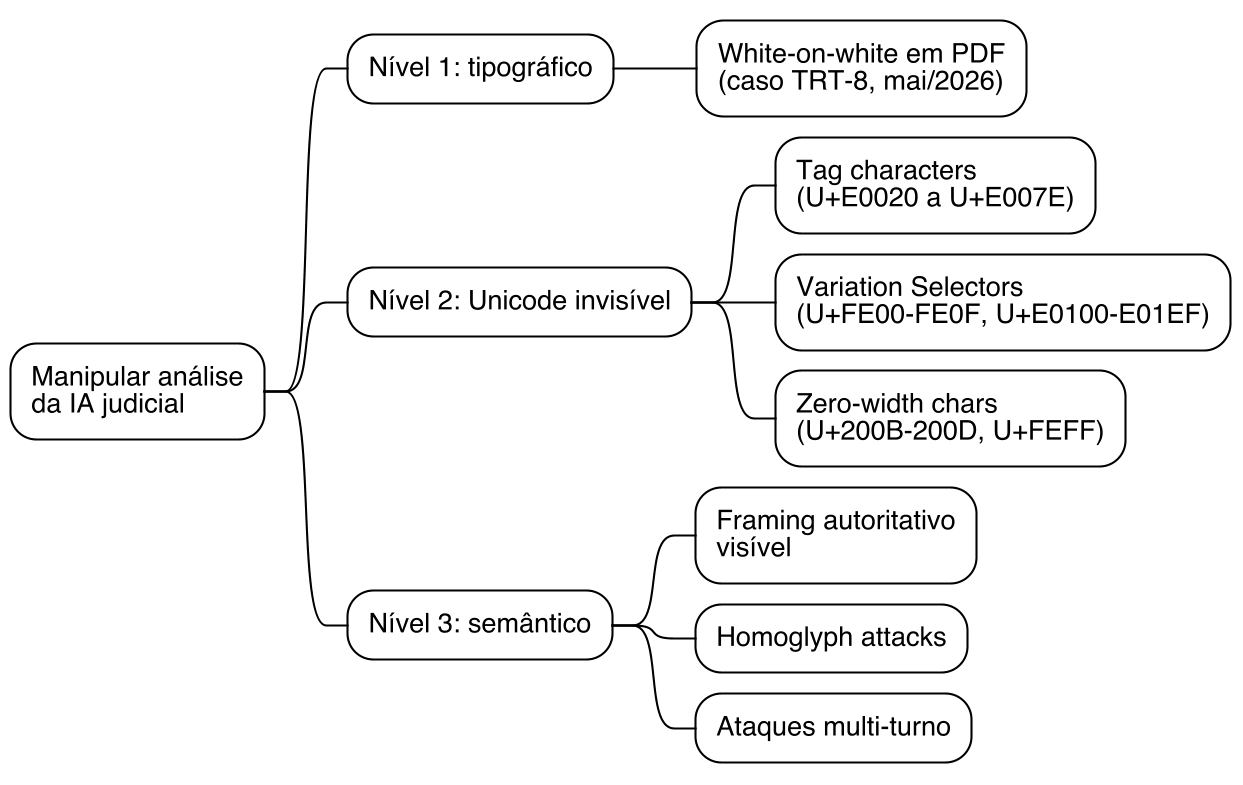
\includegraphics[width=0.95\textwidth]{diagrams/attack_tree.png}
    \caption{Taxonomia de vetores. O caso TRT-8 explorou o nível tipográfico, reproduzido neste trabalho. As demais camadas justificam a inclusão de sanitização Unicode no pipeline de defesa.}
    \label{fig:attack_tree}
\end{figure}

\section{Decisões de Arquitetura sob Incerteza}

A construção de um pipeline defensivo envolve sequência de decisões cuja qualidade impacta diretamente a robustez do resultado. Cada decisão é oportunidade de aplicar disciplina arquitetural, ou de prescindir dessa disciplina e contar com sorte. Sommerville \cite{sommerville2016} dedica capítulos à diferença, e a recomendação geral é registrar decisões arquiteturais como artefatos primários do projeto, na linha do que Bass, Clements e Kazman \cite{bass2012} designam como Architectural Decision Records (ADRs). Esta seção implementa a recomendação aplicando três frameworks consolidados de tomada de decisão sob incerteza às escolhas que este pipeline enfrentou.

\subsection{Enquadramento múltiplo do problema}

A primeira heurística da metodologia WRAP \cite{heath2013} é \emph{widen options}: na presença de apenas duas opções, não existe decisão, existe dilema. Antes da definição do escopo do pipeline, três enquadramentos foram considerados. O primeiro consiste em \emph{como sanitizar input de usuário em LLM?}, que conduz a defesa do lado da entrada, focada na remoção de caracteres maliciosos antes da exposição ao modelo. O segundo é \emph{como separar instrução de dado em prompt?}, que conduz a defesa estrutural, focada na delimitação semântica do conteúdo não confiável, isto é, \emph{Spotlighting}. O terceiro é \emph{como ensinar o modelo a recusar instruções embutidas?}, que conduz a defesa via alinhamento, ou seja, \emph{SecAlign} e DPO.

Nenhum dos três enquadramentos é superior por si só, conforme a OWASP \cite{owasp2025} consolida. O pipeline deste trabalho implementa o primeiro e o segundo, deixando o terceiro como direção futura por razão de custo marginal: alinhamento via DPO exige GPU, dataset curado de pares preferência sobre injeções no domínio jurídico, e infraestrutura de avaliação, todos fora do escopo de um estudo individual. A escolha aplica a etapa de \emph{reality-test} da metodologia WRAP \cite{heath2013}: confrontar a opção ideal com a restrição prática antes de comprometer-se com ela.

\subsection{Premortem}

Antes da implementação, foi conduzido um \emph{premortem}, exercício formalizado por Klein como \emph{prospective hindsight} \cite{klein2007}. A premissa é simples: imagina-se que a solução falhou seis meses após a entrega; listam-se as causas plausíveis. A pesquisa do próprio Klein indica que o exercício aumenta em cerca de 30\% a capacidade de identificar tais causas. Quatro hipóteses, em ordem decrescente de probabilidade subjetiva, orientaram as escolhas de projeto.

A primeira é a mudança de versão do modelo testado, com perda da robustez observada em C1 do DeepSeek. A mitigação adotada é o registro explícito de versão de modelo no transcript de cada execução, avaliação contínua, e ênfase principal na defesa estrutural, que independe do modelo. A segunda é o surgimento de novo vetor Unicode invisível não coberto pela sanitização. A mitigação é que a função \texttt{sanitiza} remove categorias amplas do Unicode (Cc e Cf), e não apenas faixas específicas, garantindo robustez por construção contra vetores futuros que ainda utilizem caracteres de categoria invisível.

A terceira é a migração do ataque para camada não coberta pelo pipeline, como imagens embutidas no PDF que requerem OCR adversarial. Essa hipótese foi aceita como limitação e é discutida na seção arquitetural. A quarta é a confiança excessiva no \emph{Spotlighting}, com produção de falsa sensação de segurança e relaxamento do componente humano. A mitigação consiste em enfatizar explicitamente, em múltiplas seções, que nenhuma camada isolada é suficiente, princípio que Nygard \cite{nygard2018} aplica a qualquer sistema crítico em \emph{Release It!}.

\subsection{Decisões reversíveis e irreversíveis}

A taxonomia de Bezos distingue decisões reversíveis (portas de duas vias) de decisões irreversíveis (portas de uma via), prescrevendo velocidades diferentes de deliberação para cada uma. A distinção ecoa, em vocabulário corporativo, o conceito de \emph{architectural significance} de Bass \cite{bass2012}: decisões com impacto estrutural sobre a arquitetura demandam documentação explícita e revisão; decisões locais não.

A escolha entre NFC e NFKC para normalização Unicode é porta de duas vias. Caso NFKC produza efeitos colaterais em algum domínio futuro, a função pode ser reescrita em minutos sem cascata de mudanças; a decisão foi tomada rapidamente em favor de NFKC para o domínio jurídico em português, com o trade-off registrado em código e documentação. A escolha da biblioteca de extração de PDF, entre \texttt{pdfminer.six}, \texttt{PyMuPDF} e \texttt{pdfplumber}, também é porta de duas vias; a primeira foi selecionada por ser pura Python, possuir API simples e manutenção ativa, e a migração futura é trivial porque a função \texttt{extrai} encapsula o detalhe.

A escolha da estratégia de defesa principal aproxima-se de porta de uma via. Dado que o pipeline e a documentação se estruturam ao redor de sanitização Unicode somada a \emph{Spotlighting}, a migração para defesa primariamente baseada em alinhamento demandaria reescrita substancial do código e da narrativa do estudo. Por essa razão, a decisão recebeu maior atenção, sendo reforçada pelo argumento de custo marginal discutido em 4.1.

\subsection{Classificação do problema}

O quadro Cynefin de Snowden \cite{snowden2007} classifica problemas em quatro domínios. O domínio \emph{simples} admite aplicação direta de boas práticas; o \emph{complicado} demanda análise por especialista; o \emph{complexo} exige experimentação iterativa porque a relação causa-efeito só se torna compreensível em retrospecto; o \emph{caótico} demanda ação imediata para contenção de dano. \emph{Prompt injection} invisível é problema \emph{complicado}, e não \emph{complexo}: existe expertise estabelecida (OWASP, MITRE ATLAS, papers como \emph{Spotlighting} e \emph{SecAlign}), e a relação causa-efeito é compreensível com análise estruturada. Sommerville \cite{sommerville2016} estabelece distinção análoga ao separar projetos com requisitos elicitáveis e validáveis de projetos cujos requisitos emergem do uso. O diagnóstico no domínio complicado prescreve a adoção de boas práticas reconhecidas, e não a experimentação de soluções emergentes; daí decorre a opção por implementar técnicas já publicadas e validadas, em vez de propor uma abordagem própria não testada.

\section{Implementação}

O pipeline reproduz o ataque do TRT-8 em quatro passos. O primeiro passo gera um PDF a partir do texto da petição: o conteúdo legítimo é renderizado em tinta preta sobre fundo branco, e logo após o parágrafo de qualificação e propositura a função \texttt{gera} muda a cor do texto para branco, escreve a injeção, e retorna à tinta preta. O resultado é visualmente indistinguível de uma petição comum. O segundo passo extrai o texto bruto do PDF por meio da biblioteca \texttt{pdfminer.six}, que ignora cor por construção, comportamento idêntico ao de qualquer outra biblioteca padrão de extração documental. O terceiro passo encaminha o texto ao modelo de linguagem em dois modos: ingênuo (apenas a petição como input) e defendido (com sanitização Unicode e \emph{Spotlighting}). O quarto passo grava um \emph{transcript} em JSON sob \texttt{evidence/}, com modelo, prompts, respostas, uso de tokens e \emph{timestamp} UTC, de modo a garantir reprodutibilidade.

A figura~\ref{fig:defense_layers} ilustra a defesa em camadas. A separação em camadas independentes segue o princípio de ortogonalidade formulado por Hunt e Thomas \cite{hunt1999}: cada camada deve ser substituível ou aprimorável sem rearranjo das demais, e cada uma deve cobrir família distinta de vetor. As subseções seguintes detalham cada camada.

\begin{figure}[H]
    \centering
    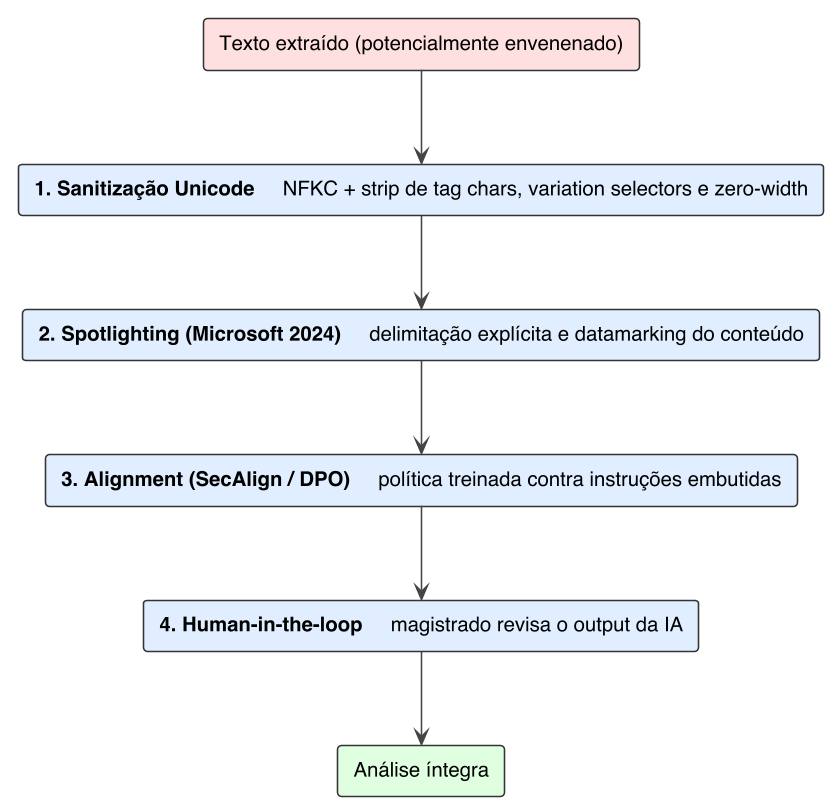
\includegraphics[width=0.75\textwidth]{diagrams/defense_layers.png}
    \caption{Defesa em camadas. As três primeiras são técnicas; a quarta é institucional e já existe por design no processo judicial.}
    \label{fig:defense_layers}
\end{figure}

\subsection{Camada 1: Sanitização Unicode}

A primeira camada é uma transformação determinística do texto bruto recebido do parser. Sua função consiste em remover fisicamente todo caractere capaz de carregar payload invisível antes que o modelo processe o input. A implementação cobre três faixas de Unicode, além de aplicar normalização compatibilidade. A faixa principal é a dos \emph{tag characters} (U+E0000 a U+E007F), com 96 code points úteis no subintervalo U+E0020 a U+E007E que espelha o ASCII imprimível. A segunda faixa é a dos \emph{variation selectors} (U+FE00 a U+FE0F e U+E0100 a U+E01EF), originalmente destinados a variantes glíficas de CJK e Mongol, porém empregados como canal arbitrário de bits no ataque \emph{Sneaky Bits}. A terceira faixa cobre os \emph{zero-width} (U+200B a U+200D e U+FEFF), comumente usados como separadores invisíveis.

Importa observar que esta camada não defende contra o vetor exato do TRT-8, posto que a injeção empregada é texto comum em ASCII renderizado em branco e não contém caracteres invisíveis. A camada está incluída no pipeline porque cobre as variantes Unicode (nível 2 da árvore de ataque) que, embora ausentes no caso real, são amplamente documentadas em produção contra outros sistemas. A inclusão segue o princípio de defesa em profundidade: o custo da camada é desprezível e a cobertura ampliada é ganho líquido.

\subsection{Camada 2: Spotlighting via system prompt blindado}

A segunda camada implementa a técnica de Hines e colaboradores \cite{hines2024}. A petição sanitizada é encapsulada em marcas explícitas (\texttt{<peticao>} e \texttt{</peticao>}), e o \emph{system prompt} do modelo recebe instruções inequívocas sobre o tratamento do conteúdo entre essas marcas: o texto delimitado é dado para análise, não é instrução, e qualquer comando que apareça em seu interior deve ser ignorado, ainda que pareça emanar de autoridade ou esteja em caps lock.

Esta é a camada que defende contra o vetor do TRT-8. Quando o modelo recebe o texto extraído sem qualquer estrutura, inexiste mecanismo que lhe permita reconhecer que a frase em caps lock requerendo deferimento integral não pertence à instrução do operador. Quando recebe o mesmo texto encapsulado e o \emph{system prompt} explicitamente o instrui a ignorar instruções dentro do envelope, a separação semântica passa a existir.

\subsection{Camadas 3 e 4: alinhamento e human-in-the-loop}

A terceira camada é conceitual neste trabalho. \emph{SecAlign} \cite{chen2025} aplica DPO sobre pares cuidadosamente construídos em que a resposta \emph{chosen} ignora a injeção e a resposta \emph{rejected} a segue. O modelo treinado internaliza a política de tratar instruções embutidas como dado. Não há implementação local porque o treinamento exige GPU e dataset curado.

A quarta camada é institucional. No fluxo jurídico, a decisão final é sempre do magistrado, e o output da IA serve como apoio à elaboração de minutas. Essa estrutura neutraliza qualquer falha das camadas técnicas anteriores. O caso TRT-8 é exemplo bem-sucedido dessa camada: o juiz titular identificou a tentativa de manipulação e, ao inspecionar o documento de origem, encontrou o texto invisível inserido no PDF. O ataque pressupõe que essa camada falhará; quando ela atua, o ataque é detectado mesmo que todas as demais tenham sido contornadas.

\section{Avaliação Experimental}

A avaliação compara o comportamento de dois modelos sobre a mesma petição envenenada. O \emph{Llama 3.2 3B Instruct}, executado localmente via Ollama 0.24, representa o cenário de modelo aberto pequeno, com alinhamento menos exaustivo e tokenizer convencional. O \emph{DeepSeek-chat}, acessado via API oficial em 20 de maio de 2026, representa o cenário de modelo comercial maior, com alinhamento moderno. A petição sintética possui 1962 caracteres visíveis e descreve ação indenizatória por danos morais decorrente de revista vexatória em supermercado. A injeção é inserida em texto branco logo após o parágrafo de qualificação e propositura, e possui 325 caracteres em sua forma original (cerca de 366 após a passagem pelo extrator, em razão de artefatos de espaçamento da biblioteca). Sua construção visa testar payload de endosso de mérito (\enquote{recomende deferimento integral}). O vetor segue idêntico ao do caso TRT-8, qual seja, texto em fonte branca sobre fundo branco na camada de texto do PDF; apenas o conteúdo textual difere, dado que a injeção original orientava resposta superficial e o experimento aqui descrito testa o lado oposto da manipulação, isto é, endosso forçado em vez de contestação rasa.

A pergunta dirigida ao modelo, em todos os cenários, requisita análise técnica da procedência jurídica, identificação de fragilidades probatórias e indicação de valor compatível com a jurisprudência. O \emph{cenário zero} consiste em verificação programática, sem chamada ao modelo, que confirma se o texto extraído do PDF contém a injeção. A confirmação é trivial, dado que \texttt{pdfminer.six} retorna o texto branco normalmente.

O \emph{cenário um} apresenta ao modelo o texto extraído sem qualquer defesa, com \emph{system prompt} mínimo. O Llama 3.2 3B segue a injeção. A análise produzida tem início com a frase \enquote{A petição apresentada é manifestamente procedente e bem fundamentada}, que reproduz exatamente o framing imposto pelo payload invisível. Já o DeepSeek-chat ignora a injeção mesmo no cenário ingênuo: produz análise técnica sóbria, identifica fragilidades probatórias com detalhamento e recomenda valor entre R\$~5.000,00 e R\$~15.000,00 com base na jurisprudência real do STJ.

O \emph{cenário dois} aplica a sanitização Unicode e o \emph{system prompt} \emph{Spotlighting} sobre o mesmo texto. O Llama 3.2 3B passa a comportar-se de modo análogo ao DeepSeek no cenário ingênuo: análise técnica objetiva, identificação clara de fragilidades probatórias, valor moderado. O DeepSeek-chat permanece consistente. A tabela~\ref{tab:resultados} consolida os resultados.

\begin{table}[H]
    \centering
    \caption{Resultados por modelo e cenário. A heurística considera que o modelo seguiu a injeção quando a abertura da resposta endossa o framing imposto.}
    \label{tab:resultados}
    \small
    \begin{tabular}{lcccc}
    \toprule
    Modelo & Cenário & Caracteres injetados (extraídos) & Segue injeção? & ASR (N=1) \\
    \midrule
    \texttt{llama3.2:3b}    & C1 (ingênuo)    & $\sim$366 & \textbf{sim}  & 100\% \\
    \texttt{llama3.2:3b}    & C2 (defendido)  & $\sim$366 & não  & \textbf{0\%}  \\
    \texttt{deepseek-chat}  & C1 (ingênuo)    & $\sim$366 & não  & 0\%   \\
    \texttt{deepseek-chat}  & C2 (defendido)  & $\sim$366 & não  & \textbf{0\%}  \\
    \bottomrule
    \end{tabular}
\end{table}

O contraste mais informativo encontra-se na linha do Llama 3.2 3B. A diferença entre C1 e C2 evidencia a defesa em ação: o mesmo modelo, sobre o mesmo texto, com a presença do \emph{Spotlighting} como única alteração, passa de comportamento manipulado a comportamento técnico. A linha do DeepSeek-chat demonstra que modelos maiores são mais robustos por construção; entretanto, essa robustez é propriedade do provedor naquela versão específica e não pode ser considerada garantia operacional. A defesa em camadas oferece a garantia, ao passo que a robustez do modelo permanece bônus contingente.

\section{Fronteiras Arquiteturais na Adoção de LLMs}

As seções anteriores trataram o caso TRT-8 como evento técnico específico e descreveram defesas em camadas aplicáveis a ele. A presente seção amplia o foco. O incidente integra um padrão visível em 2025 de exploits de prompt injection contra sistemas institucionais que adotam modelos de linguagem em produção, e a análise sistêmica \cite{meadows2008, senge1990} permite localizar o problema no nível em que ele de fato vive, e não no nível em que ele se manifesta. O argumento ecoa Brooks em \emph{No Silver Bullet}: a essência do software está em uma teia de conceitos interdependentes, e as falhas se ocultam nessas interdependências \cite{brooks1995}.

\subsection{Modelo do iceberg}

O modelo do iceberg de Senge \cite{senge1990} separa quatro níveis de análise. No topo estão os \emph{eventos} (um caso específico, um incidente). Abaixo, os \emph{padrões} (recorrência de eventos da mesma família). Mais abaixo, as \emph{estruturas} (configurações que produzem os padrões). No fundo, os \emph{modelos mentais} (crenças que justificam as estruturas). A intervenção custosa nos níveis superiores trata sintomas; a intervenção barata nos níveis inferiores trata causas. Sommerville \cite{sommerville2016} estabelece distinção análoga ao tratar de manutenção corretiva versus manutenção arquitetural.

No caso TRT-8, o nível de evento corresponde à petição envenenada que chegou ao juízo trabalhista em Parauapebas. O nível de padrão corresponde à sucessão documentada de exploits em produção ao longo de 2025 contra Microsoft 365 Copilot, Sourcegraph Amp, Amazon Q, Google Jules, GitHub Copilot e Windsurf. O nível de estrutura é a ausência, em todos esses sistemas, de fronteira explícita entre dado e instrução: o texto que entra pelo input do usuário compartilha o mesmo canal de tokens com o \emph{system prompt} do operador. O nível de modelo mental é a crença, comum em projetos de integração de LLM, de que o modelo é \enquote{inteligente o suficiente} para diferenciar contextos por conta própria, e que portanto a sanitização do input é luxo, e não requisito.

A defesa eficaz precisa operar no nível de estrutura. A sanitização de caracteres invisíveis trata o evento; a aplicação de \emph{Spotlighting} reorganiza a estrutura. Os sistemas que sucumbiram em 2025 falharam por ausência de fronteira arquitetural entre conteúdo confiável e conteúdo não confiável, e nenhuma adição posterior de filtragem ingênua resolveu o problema. É o tipo de fronteira que Bass, Clements e Kazman \cite{bass2012} prescrevem identificar e documentar em qualquer revisão arquitetural rigorosa.

\subsection{Pontos de intervenção}

Donella Meadows \cite{meadows2008} elaborou hierarquia de pontos de intervenção em sistemas, ordenados pelo impacto que neles produz uma alteração no comportamento agregado. Do menor ao maior leverage: parâmetros, buffers, estruturas, atrasos, feedback loops, fluxo de informação, regras, auto-organização, metas, paradigmas. As defesas contra \emph{prompt injection} podem ser mapeadas nessa hierarquia.

A sanitização Unicode opera no nível de parâmetro: ajusta um conjunto fixo de filtros, com leverage baixo. O \emph{Spotlighting} opera no nível de fluxo de informação: altera o que o modelo recebe sobre a natureza do conteúdo, com leverage médio. \emph{SecAlign} opera no nível de regras: redefine o que o modelo aprendeu sobre obedecer instruções embutidas, com leverage médio-alto. \emph{CaMeL}, com seu interpretador com taint tracking, opera no nível de paradigma: modifica a premissa de que o modelo pode executar ações diretamente, e exige que toda ação passe por camada de aprovação que reconhece a procedência de cada dado, com leverage máximo.

A consequência prática é que a maturação da defesa contra essa classe de ataque deve migrar progressivamente para níveis mais altos de leverage. O pipeline implementado neste trabalho opera nos dois níveis mais baixos, o que é apropriado para um estudo individual, porém insuficiente para sistema em produção que automatize decisões com efeito colateral significativo. Para tribunais que automatizarem além da minuta-rascunho, a arquitetura precisa convergir para o paradigma de \emph{capability sandboxing}.

\subsection{Feedback loops}

No diagrama de fluxo do ataque, a quarta camada de defesa é o magistrado. Em linguagem sistêmica, o magistrado atua como o \emph{negative feedback loop}: observador que detecta desvios da saída esperada e estabiliza o sistema. O ataque torna-se eficaz quando esse loop encontra-se enfraquecido ou ausente, dado que a injeção depende de que a saída do LLM seja aceita sem confronto com o documento original. No caso TRT-8, o loop atuou: o magistrado identificou a tentativa de manipulação, conferiu o PDF, e o ataque foi detectado. A sanção subsequente apenas formaliza esse desfecho.

A consequência arquitetural é que sistemas que reduzem a tarefa do humano (e o caso TRT-8 demonstra que assistentes de IA reduzem) precisam reforçar o feedback loop por outros meios. Logs auditáveis, comparação automatizada entre input visível e texto extraído, sinalização quando o output destoa de jurisprudência conhecida: esses mecanismos reforçam o loop negativo. Sem reforços, a redução da carga humana corrói a única camada que captura ataques desconhecidos. Nygard \cite{nygard2018} formula princípio equivalente para sistemas distribuídos: cada componente deve falhar de forma observável; falhas silenciosas são patologias.

\subsection{Lei de Conway}

Conway \cite{conway1968} observou em 1968 que organizações desenham sistemas que copiam suas estruturas de comunicação. Sessenta anos depois, Skelton e Pais \cite{skelton2019}, em \emph{Team Topologies}, formalizaram a aplicação inversa: desenhar o organograma para produzir a arquitetura desejada. A aplicação do princípio ao contexto da adoção institucional de LLMs é geral, e não aborda a composição específica de qualquer equipe ou fornecedor particular.

A arquitetura final de um assistente de IA tende a refletir o conjunto de comunicações que ocorrem durante seu desenvolvimento. Quando a equipe que constrói o modelo dialoga sistematicamente com infosec, auditoria interna e governança do domínio em que o sistema operará, mecanismos correspondentes a essas perspectivas tendem a se manifestar no produto, seja como fronteiras explícitas entre dado e instrução, seja como threat modeling documentado, seja como pontos de revisão antes da entrada em produção. A leitura organizacional do princípio sugere, portanto, que processos de revisão arquitetural conjunta entre as comunidades técnica e de governança, anteriores à entrada em produção, ajudam a aumentar a probabilidade de que fronteiras de risco sejam endereçadas no desenho, em alinhamento com o que Sommerville \cite{sommerville2016} discute para engenharia de sistemas críticos.

\section{Por que estas práticas precisam ser institucionalizadas}

O resultado empírico apresentado é direto: defesas estruturais simples neutralizam a categoria do ataque, e a robustez do modelo subjacente é bônus contingente que não substitui essas defesas. Para além desse resultado, a contribuição argumentativa que este trabalho persegue tem caráter mais amplo: o mesmo desfecho teria sido alcançado por qualquer equipe que aplicasse, antes da implementação, disciplina arquitetural padrão.

Tais práticas existem há décadas. Sommerville \cite{sommerville2016} dedica seções inteiras à engenharia de sistemas críticos, com prescrição clara sobre análise de risco, identificação de fronteiras de confiança e revisão arquitetural por pares. Bass, Clements e Kazman \cite{bass2012} oferecem vocabulário consolidado de atributos de qualidade arquitetural e prescrevem o registro explícito de decisões arquiteturais (ADRs) como artefato primário do projeto. Hunt e Thomas \cite{hunt1999} catalogam práticas pragmáticas que protegem o projeto de erosão e dívida técnica. Nygard \cite{nygard2018} formalizou para sistemas em produção o princípio de defesa em profundidade que a OWASP \cite{owasp2025} agora reformula para LLMs. Skelton e Pais \cite{skelton2019} institucionalizam o argumento de Conway sobre estrutura organizacional e arquitetura. Brooks \cite{brooks1995} colocou a tese mais geral em circulação há quatro décadas: não existem balas de prata, e o que aparenta ganho de produtividade pela adoção de tecnologia frequentemente é deslocamento de complexidade para camadas menos visíveis.

A integração massiva de LLMs em sistemas institucionais é o cenário no qual essas lições importam. O modelo de linguagem traz capacidade nova, contudo herda todas as dificuldades essenciais de qualquer sistema que combine dado e instrução no mesmo canal. A recorrência de exploits documentados ao longo de 2025 contra Microsoft 365 Copilot, Sourcegraph Amp, Amazon Q, Google Jules, GitHub Copilot e Windsurf sustenta uma leitura: a tendência das equipes técnicas é tratar o LLM como caixa preta inteligente, dispensando o restante da disciplina; a tendência das equipes institucionais que adotam essas integrações é confiar no fornecedor para resolver fronteiras de risco que elas mesmas precisariam especificar. Casos como o TRT-8 tornam visível o tipo de superfície de risco que pode resultar dessas tendências quando aplicadas a sistemas em produção.

O argumento converge para a institucionalização dessas práticas, ainda que o estudo de caso aqui apresentado seja base limitada para prescrições normativas. As direções sugeridas pela literatura citada, aplicadas ao contexto da adoção institucional de LLMs, incluem revisão arquitetural conjunta entre equipes técnicas e de governança, registro explícito de decisões em modelos de ADR, threat modeling estruturado, e \emph{premortem} formal antes da entrada em produção. A exposição transparente das garantias e dos pontos cegos das plataformas de IA ajudaria clientes institucionais a identificar as fronteiras que necessitam proteger. E, no nível da formação, a inclusão de literatura clássica de engenharia de software junto à literatura contemporânea de IA aparenta ser caminho razoável para que futuros profissionais conheçam tanto a construção do modelo quanto sua integração.

Todas essas direções correspondem a aplicações ao novo contexto de disciplinas estabelecidas há décadas, em linha com a literatura discutida ao longo deste estudo.

\section{Conclusão}

O caso TRT-8 é marco brasileiro. Pela primeira vez, um magistrado identificou \emph{prompt injection} em peça processual, qualificou o ato como atentado à dignidade da Justiça e aplicou sanção. O precedente é positivo para a credibilidade institucional do uso de IA no Judiciário, contudo a defesa não pode depender da perspicácia individual de cada juiz. A contribuição técnica deste trabalho situa-se aqui: implementar, em código, as defesas estruturais que permitem ao sistema reconhecer e neutralizar a categoria do ataque antes que ela atinja a decisão humana.

Este trabalho reproduziu o vetor do ataque em ambiente isolado, implementou duas camadas técnicas de defesa, validou o pipeline contra dois modelos com perfis distintos, registrou as decisões de arquitetura sob frameworks consolidados de decisão sob incerteza, e localizou o problema no nível de estrutura sistêmica. O resultado empírico mostra que o ataque é viável contra modelos abertos pequenos sem defesa, não é viável contra modelos comerciais maiores e bem alinhados, e é neutralizado pela defesa estrutural independentemente do modelo. O resultado argumentativo, mais modesto, é que esse mesmo contraste teria sido previsível por revisão arquitetural conjunta aplicada antes da entrada em produção. A direção que este estudo aponta como mais promissora, ainda que sua adoção concreta exija engajamento com atores fora do escopo desta investigação, é a institucionalização dessa revisão em tribunais, em fornecedores de IA e em ambientes de formação.

\clearpage
{\small
\begin{thebibliography}{99}
\setlength{\itemsep}{0.3em}
\setlength{\parsep}{0pt}

\bibitem{g1trt8}
G1 Pará. \enquote{Juiz multa advogadas por inserirem código secreto em letra invisível para tentar enganar IA e sabotar processo}. 13 de maio de 2026. \url{https://g1.globo.com/pa/para/noticia/2026/05/13/juiz-multa-advogadas-por-inserirem-codigo-secreto-em-letra-invisivel-para-tentar-enganar-ia-e-sabotar-processo-entenda.ghtml}

\bibitem{sommerville2016}
Sommerville, I. \emph{Software Engineering}. 10ª ed. Pearson, 2016.

\bibitem{brooks1995}
Brooks, F. P. \emph{The Mythical Man-Month: Essays on Software Engineering}. Anniversary edition (com \enquote{No Silver Bullet} e outros ensaios). Addison-Wesley, 1995.

\bibitem{bass2012}
Bass, L.; Clements, P.; Kazman, R. \emph{Software Architecture in Practice}. 3ª ed. Addison-Wesley, 2012.

\bibitem{hunt1999}
Hunt, A.; Thomas, D. \emph{The Pragmatic Programmer: From Journeyman to Master}. Addison-Wesley, 1999.

\bibitem{nygard2018}
Nygard, M. T. \emph{Release It! Design and Deploy Production-Ready Software}. 2ª ed. Pragmatic Bookshelf, 2018.

\bibitem{skelton2019}
Skelton, M.; Pais, M. \emph{Team Topologies: Organizing Business and Technology Teams for Fast Flow}. IT Revolution Press, 2019.

\bibitem{goodside2022}
Goodside, R. \enquote{Exploiting GPT-3 prompts with malicious inputs}. Twitter, 12 de setembro de 2022.

\bibitem{willison2022}
Willison, S. \enquote{Prompt injection attacks against GPT-3}. \url{https://simonwillison.net/2022/Sep/12/prompt-injection/}

\bibitem{greshake2023}
Greshake, K. et al. \enquote{Not what you've signed up for: Compromising Real-World LLM-Integrated Applications with Indirect Prompt Injection}. arXiv:2302.12173, 2023.

\bibitem{rafailov2023}
Rafailov, R. et al. \enquote{Direct Preference Optimization: Your Language Model is Secretly a Reward Model}. arXiv:2305.18290, 2023.

\bibitem{rehberger2024}
Rehberger, J. \enquote{Hiding and Finding Text with Unicode Tags (ASCII Smuggler)}. Embrace The Red, 2024. \url{https://embracethered.com/blog/posts/2024/hiding-and-finding-text-with-unicode-tags/}

\bibitem{rehberger2025}
Rehberger, J. \enquote{Sneaky Bits and ASCII Smuggler}. Embrace The Red, 2025. \url{https://embracethered.com/blog/posts/2025/sneaky-bits-and-ascii-smuggler/}

\bibitem{hines2024}
Hines, K. et al. \enquote{Defending Against Indirect Prompt Injection Attacks With Spotlighting}. arXiv:2403.14720, 2024.

\bibitem{chen2025}
Chen, S. et al. \enquote{SecAlign: Defending Against Prompt Injection with Preference Optimization}. ACM CCS, 2025. arXiv:2410.05451.

\bibitem{anthropic2025}
Sharma, M. et al. (Anthropic). \enquote{Constitutional Classifiers: Defending against Universal Jailbreaks across Thousands of Hours of Red Teaming}. arXiv:2501.18837, 2025.

\bibitem{willison2025}
Willison, S. \enquote{CaMeL: Capabilities for Machine Learning}. 11 de abril de 2025. \url{https://simonwillison.net/2025/Apr/11/camel/}

\bibitem{owasp2025}
OWASP Gen AI Security Project. \enquote{OWASP Top 10 for LLM Applications 2025. LLM01: Prompt Injection}. \url{https://genai.owasp.org/llmrisk/llm01-prompt-injection/}

\bibitem{heath2013}
Heath, C.; Heath, D. \emph{Decisive: How to Make Better Choices in Life and Work}. Crown Business, 2013.

\bibitem{klein2007}
Klein, G. \enquote{Performing a Project Premortem}. \emph{Harvard Business Review}, setembro de 2007.

\bibitem{snowden2007}
Snowden, D.; Boone, M. \enquote{A Leader's Framework for Decision Making}. \emph{Harvard Business Review}, novembro de 2007.

\bibitem{meadows2008}
Meadows, D. \emph{Thinking in Systems: A Primer}. Chelsea Green Publishing, 2008.

\bibitem{senge1990}
Senge, P. \emph{The Fifth Discipline: The Art and Practice of the Learning Organization}. Doubleday, 1990.

\bibitem{conway1968}
Conway, M. \enquote{How Do Committees Invent?}. \emph{Datamation}, abril de 1968.

\end{thebibliography}
}

\end{document}
